\section{Azioni globali}
Di seguito le azioni che possono essere effettuate in qualsiasi modalità di creazione di diagrammi.

\subsection{Esportazione file Java}
Per salvare il progetto in uso, dal menu superiore, all'interno della voce \textit{File} selezionare \textit{Esporta}.\\
\begin{figure}[H]
	\centering
		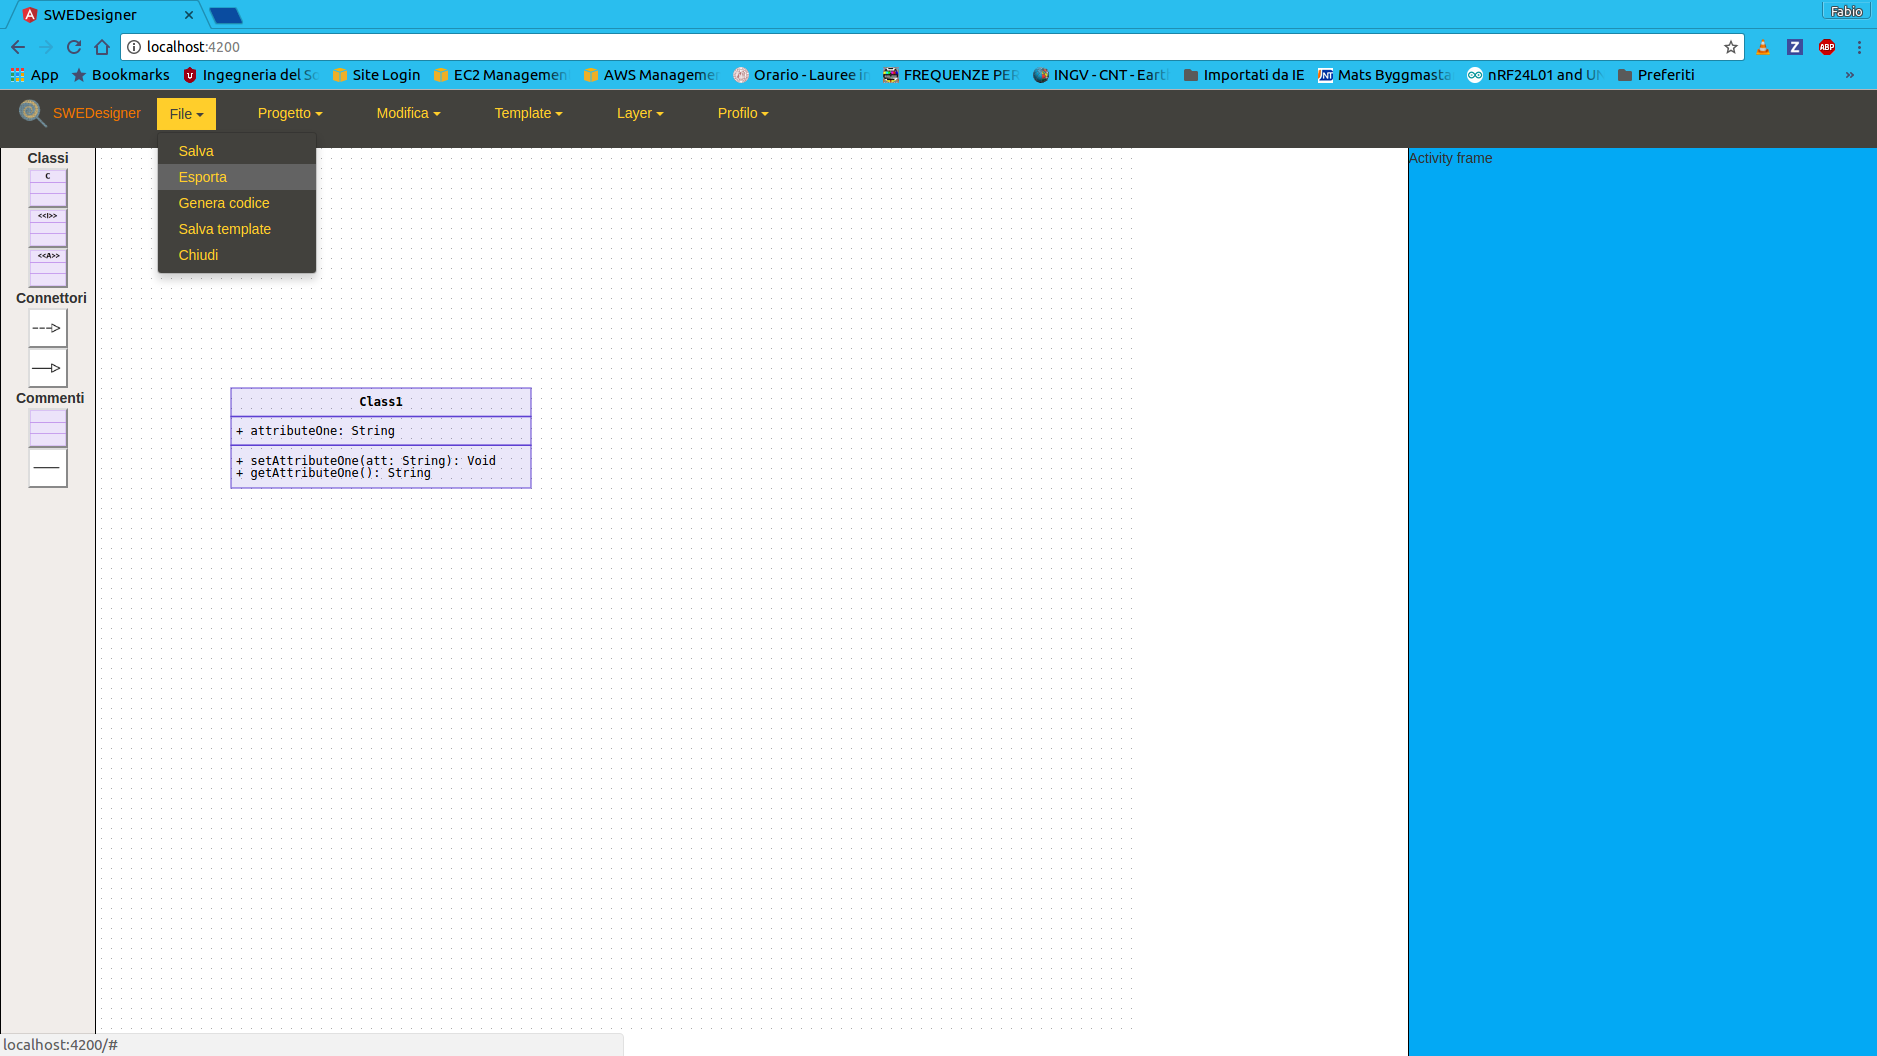
\includegraphics[width=1\linewidth]{res/img/esporta.png}
	\caption{Esportazione codice sorgente Java}
\end{figure}
\newpage

\subsection{Annulla ultima azione}
Per eliminare l'ultima azione eseguita occorre andare all'interno della voce \textit{Modifica} del menu superiore e selezionare \textit{Annulla}.\\
\begin{figure}[H]
	\centering
		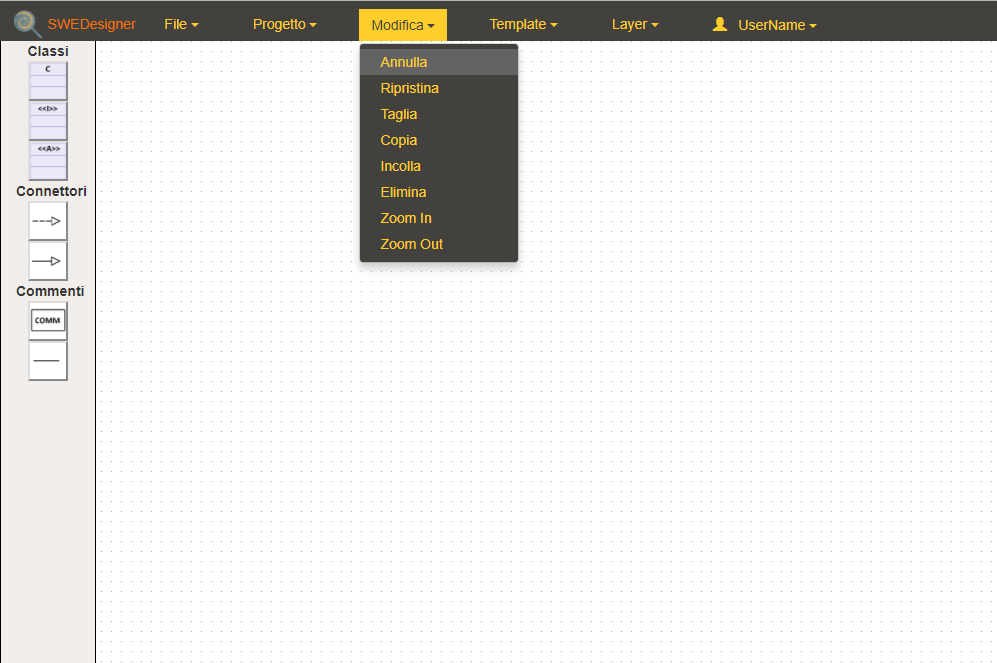
\includegraphics[width=1\linewidth]{res/img/annulla.png}
	\caption{Annulla ultima azione}
\end{figure}
\newpage

\subsection{Ripristina azione annullata}
Per ripristinare un azione che è appena stata annullata occorre andare all'interno della voce \textit{Modifica} del menu superiore e selezionare \textit{Ripristina}.

\subsection{Taglia}
Per tagliare un elemento occorre selezionarlo e successivamente andare all'interno della voce \textit{Modifica} del Menu e selezionare \textit{Taglia}.\\
\begin{figure}[H]
	\centering
		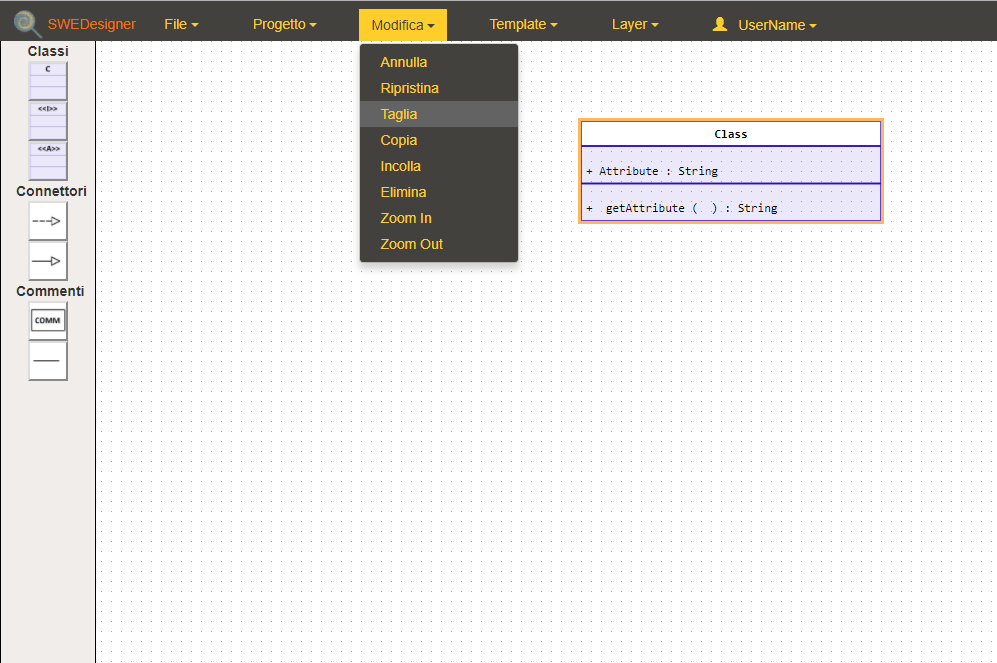
\includegraphics[width=1\linewidth]{res/img/taglia.png}
	\caption{Taglia}
\end{figure}
\newpage

\subsection{Copia}
Per copiare un elemento occorre selezionarlo e successivamente andare all'interno della voce \textit{Modifica} del Menu e selezionare \textit{Copia}.\\
\begin{figure}[H]
	\centering
		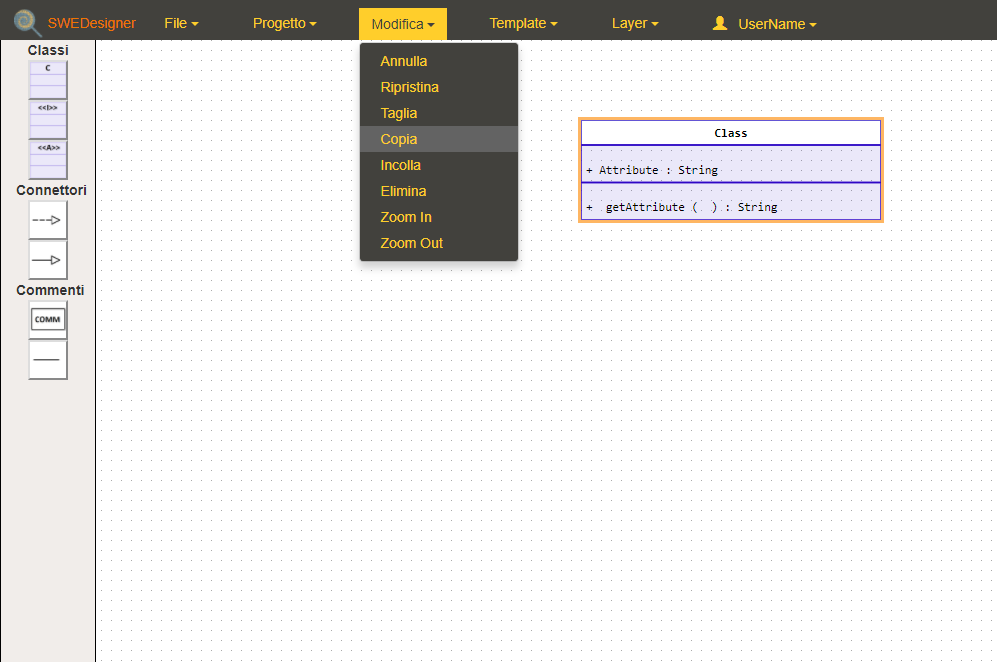
\includegraphics[width=1\linewidth]{res/img/copia.png}
	\caption{Copia}
\end{figure}
\newpage

\subsection{Incolla}
Per incollare un elemento occorre selezionarlo e successivamente andare all'interno della voce \textit{Modifica} del Menu e selezionare \textit{Incolla}. L'elemento precedentemente copiato o tagliato sarà quindi incollato sullo stesso punto in cui era stato copiato o tagliato, andando eventualmente a sovrapporsi all'elemento copiato, rimanendo riconoscibile grazie al nome modificato.\\
\begin{figure}[H]
	\centering
		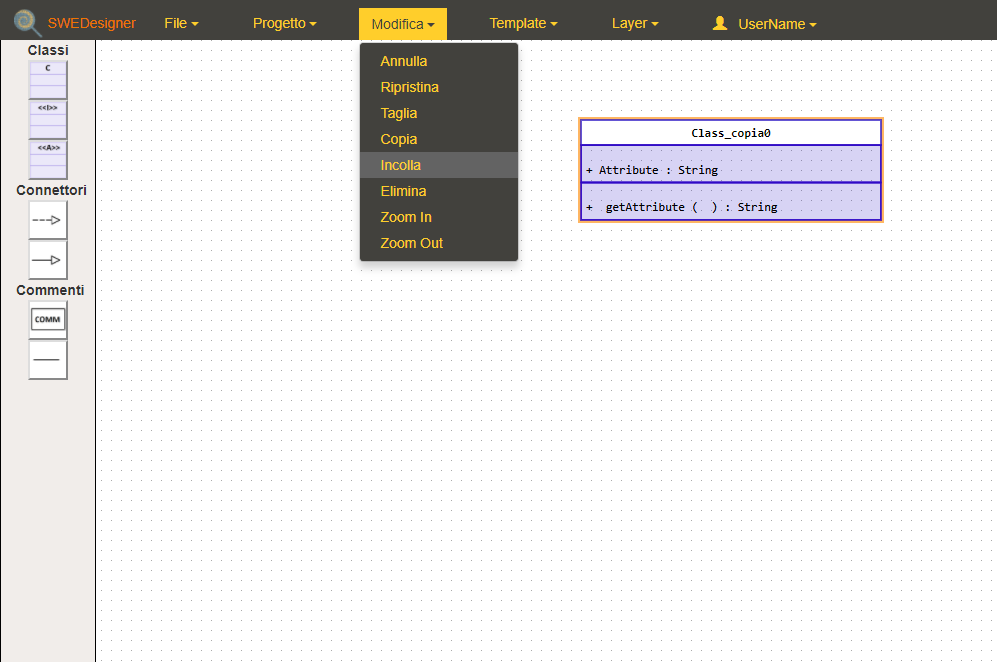
\includegraphics[width=1\linewidth]{res/img/incolla.png}
	\caption{Incolla}
\end{figure}
\newpage

\subsection{Eliminazione elemento}
Per eliminare un elemento disegnato, ma non desiderato, occorre selezionare l'elemento, e dal menu superiore, all'interno della voce \textit{Modifica} selezionare \textit{Elimina}.\\
\begin{figure}[H]
	\centering
		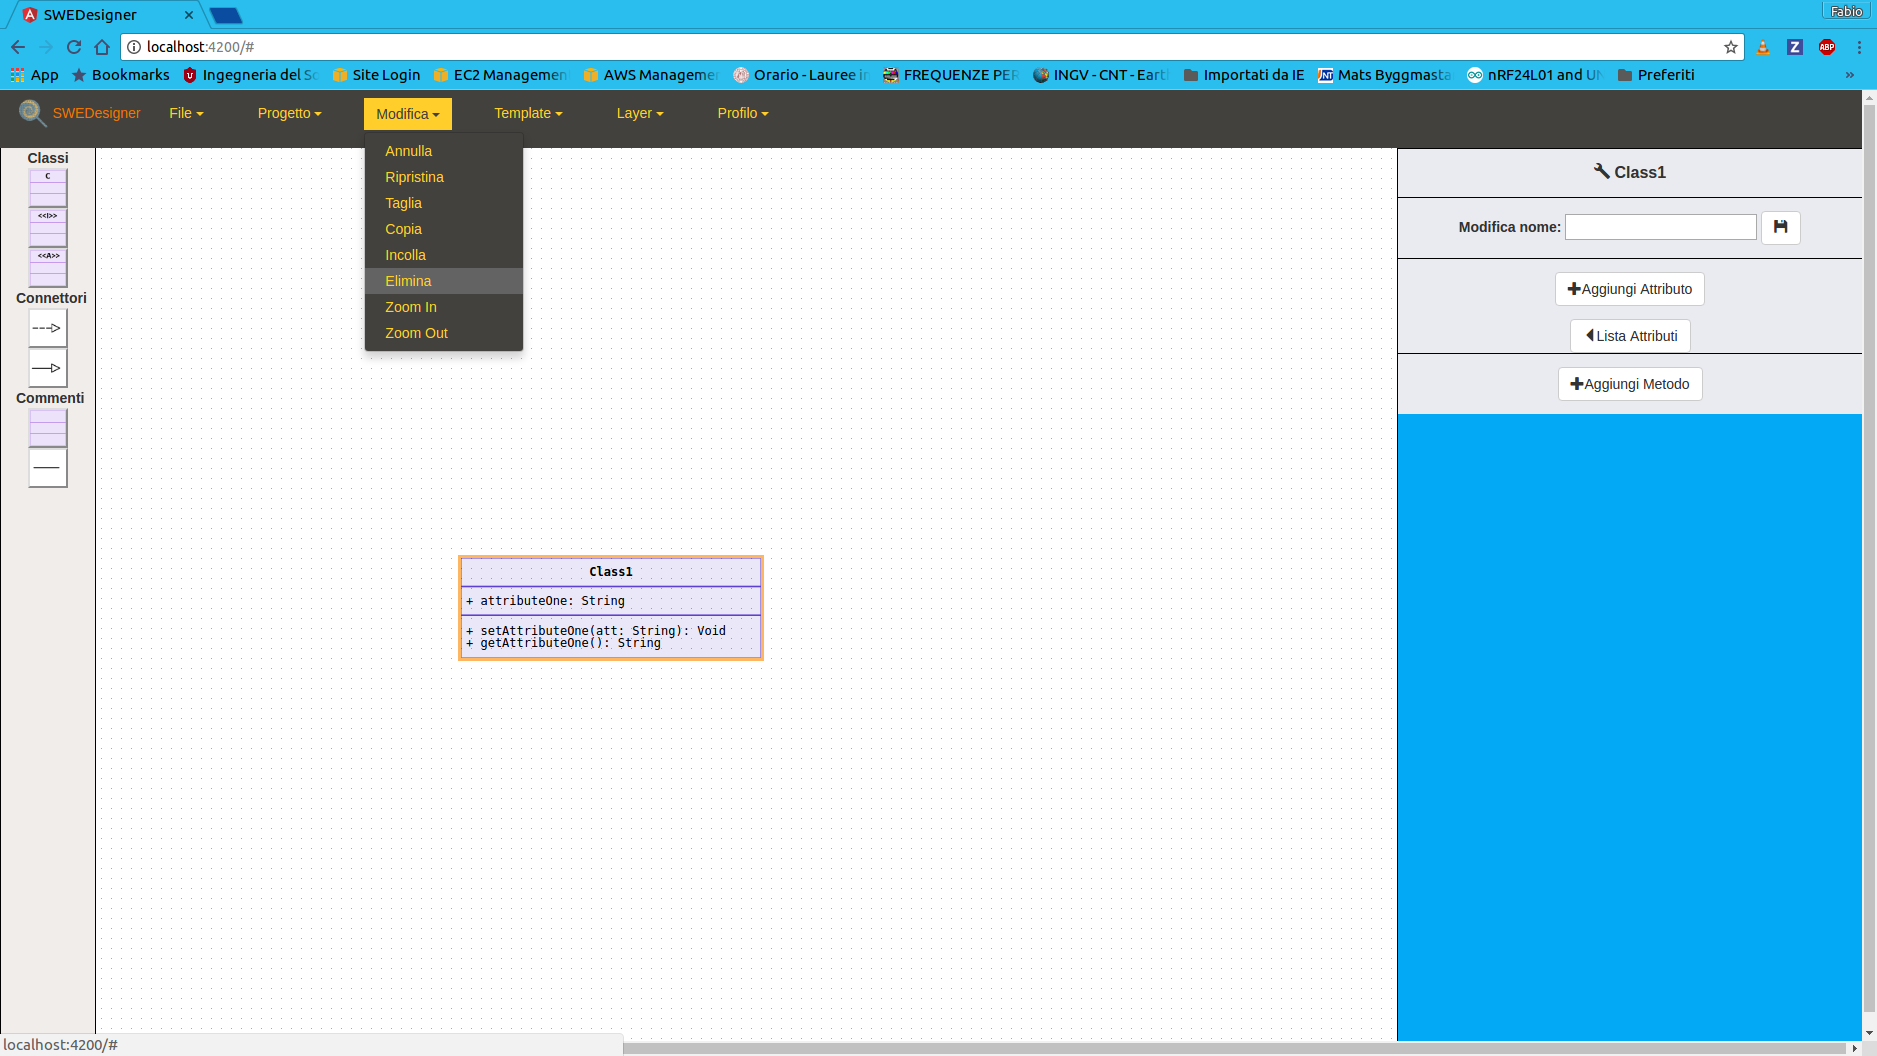
\includegraphics[width=1\linewidth]{res/img/elimina.png}
	\caption{Elimina}
\end{figure}
\newpage

\subsection{Operazioni di Zoom}
Per effettuare le operazioni di zoom dei diagrammi selezionare dal menu superiore, all'interno della voce \textit{Modifica} selezionare \textit{Zoom In} oppure \textit{Zoom Out}.\
\begin{figure}[H]
	\centering
		\includegraphics[width=1\linewidth]{res/img/zoom.png}
	\caption{Zoom}
\end{figure}
\newpage

\subsection{Associazioni tra elementi}
Per realizzare una associazione tra due elementi, una volta selezionato il tipo di relazione dal menu laterale di sinistra, bisogna cliccare prima sul elemento di partenza e successivamente sul elemento di destinazione. In seguito verrà visualizzata la freccia rappresentante l'associazione tra gli elementi.\\
\begin{figure}[H]
	\centering
		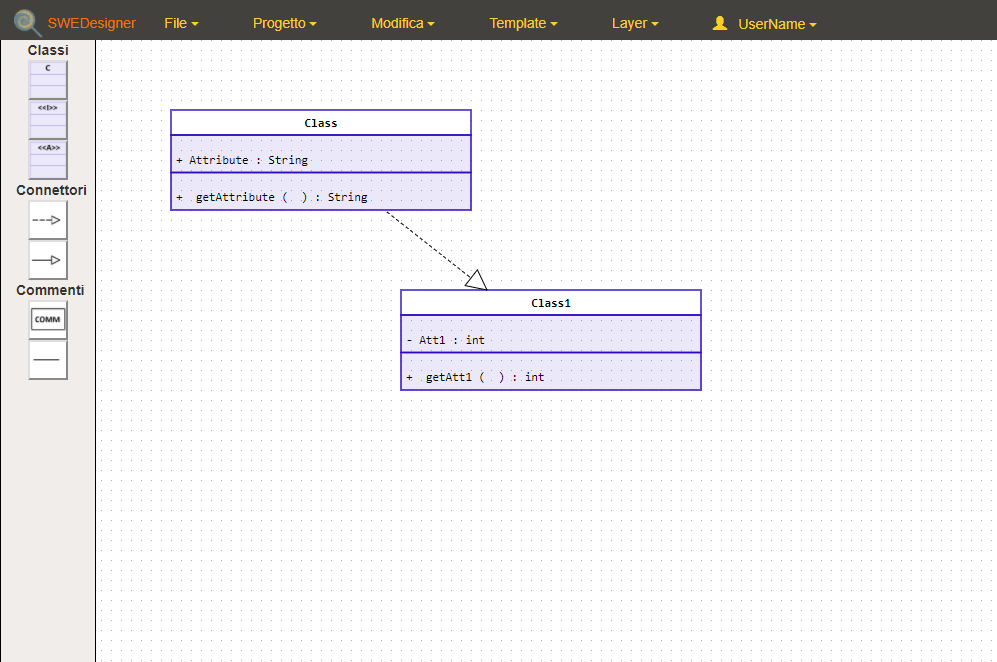
\includegraphics[width=1\linewidth]{res/img/associazioneElementi.png}
	\caption{Associazione Elementi}
\end{figure}